\section{Geometry of implicit curves}
We have played around now with the graphs of functions; these are a very important class of curve, but many useful
curves are \emph{not} graphs of functions. For example, the two curves displayed in figure \ref{fig:implicit1} are
not graphs of functions as they do not satisfy the `vertical line test'.
%   x^2 + y^2 = 25 \text{ and } x^3 + y^4 = 5xy - 2x

\begin{figure}
  \centering
  \begin{tikzpicture}
    \begin{axis}[
      axis lines = center,
      axis equal,
      xlabel = $ x $,
      ylabel = {$ y $},
    ]
    \addplot +[no markers,
      raw gnuplot,
      color=black,
      empty line = jump % not strictly necessary, as this is the default behaviour in the development version of PGFPlots
      ] gnuplot {
      set contour base;
      set cntrparam levels discrete 0.003;
      unset surface;
      set view map;
      set isosamples 100;
      set samples 100;
      splot x^2 + y^2 - 25;
    };
    \addplot +[no markers,
      raw gnuplot,
      color=red,
      empty line = jump % not strictly necessary, as this is the default behaviour in the development version of PGFPlots
      ] gnuplot {
      set contour base;
      set cntrparam levels discrete 0.003;
      unset surface;
      set view map;
      set isosamples 100;
      set samples 100;
      splot x^3 + y^4 - 5*x*y + 2*x;
    };
    \end{axis}
  \end{tikzpicture}
  \caption{Two curves, which are not graphs of functions.\label{fig:implicit1}}
\end{figure}

The two curves were generated by plotting the set of all points $ (x,y) $ satisfying the following equations:
\begin{align*}
  x^2 + y^2 - 25 &= 0; \tag{black}\\
  x^3 + y^4 - 5xy + 2x &= 0. \tag{red}
\end{align*}

This suggests that we should expand our definition of `graph' from merely functions to arbitrary equations in two variables:-
\begin{defn}
  Let $ f $ be a function of two variables; in other words, a function which takes two arguments, which we will usually call $ x $ and $ y $
  (the value of $ f $ at this pair of arguments is written $ f(x,y) $). Then the \emph{implicit curve generated by $ f $} is the set of all
  points $ (x,y) $ such that $ f(x,y) = 0 $.
\end{defn}

For example, our two curves above are the implicit curves generated by the two functions
\begin{align*}
  f(x,y) &= x^2 + y^2 - 25 \text{ and} \tag{black}\\
  g(x,y) &= x^3 + y^4 - 5xy + 2x. \tag{red}
\end{align*}

We would like to be able to talk about the geometry of curves like this using similar language to the language we have already developed; we would
like to be able to say that the black circle has negative slope at $ (4,3) $ and positive slope at $ (4,-3) $ for example.

Luckily if our curve of interest is `sufficiently nice' at a given point $ (x_0,y_0) $ (follow the footnote for the technical meaning of this, though
basically every simple thing you write down will be nice enough for us --- we need the curve to be non-vertical, not cross itself, and not be too
wiggly)\footnote{The function $ f $ needs to satisfy the hypotheses of the implicit function theorem; we need $ f $ to be continuously differentiable
and we need $ \pd{f}{y} \neq 0 $ at every point of interest, i.e. the curve cannot be vertical there.}
then a theorem called the \emph{implicit function theorem} tells us that there is a function whose graph coincides with the curve around the point. In
other words, if we have an implicit curve generated by $ f $, and $ f $ is nice at $ (x_0,y_0) $, then there exists some function $ \hat f $ defined
around $ x_0 $ such that whenever $ x $ is very close to $ x_0 $, $ (x,\hat f(x)) $ is on the curve. Since $ \hat f $ is differentiable in the usual way,
and has a graph with the same shape as the curve at $ (x_0,y_0) $, it is reasonable to define the slope of the curve at $ (x_0, y_0) $ (which we will
call $ \eval{\od{y}{x}}_{(x_0,y_0)} $) to be the slope of the graph of $ \hat f $ at $ x_0 $. In other words,
\begin{equation}
  \eval{\od{y}{x}}_{(x_0,y_0)} := \hat f'(x_0).
\end{equation}

Stop and reread the above paragraph. Draw some pictures and convince yourself that the idea makes intuitive sense (you should be able to see that,
geometrically, it makes sense). We will not prove the implicit function theorem, but you need to convince yourself that it is plausible.

We therefore have reduced our problem to finding this function $ \hat f $. I will illustrate our general technique through a couple of examples.

\begin{ex}
  Consider the circle, $ x^2 + y^2 = 25 $; let us differentiate it at $ A = (4,3) $ and $ B = (4,-3) $. The implicit function theorem tells us that there
  exist two functions, $ f $ and $ g $, such that the graph of $ f $ is precisely some part of the circle around $ A $ and such that the graph of $ G $
  is precisely some part of the circle around $ B $.

  Let us take $ f $ first. We have that $ x^2 + f(x)^2 = 25 $; we can differentiate both sides with respect to $ x $, obtaining that $ 2x + 2f(x) f'(x) = 0 $
  (we need to use the chain rule to find $ \od{}{x} [f(x)^2] $) and hence $ f'(x) = \frac{-2x}{2f(x)} $. But we are interested in $ x = 4 $; and by definition
  of $ f $, we have $ f(4) = 3 $ (since $ f $ has the same graph as the curve around $ (4,3) $); so $ f'(4) = \frac{-2 \cdot 4}{2 \cdot 3} = -\frac{4}{3} $.
  This is negative, as we expected.

  For the case of point $ B $, the same calculation tells us that $ g'(x) = \frac{-2x}{2g(x)} $ and so $ g'(4) = \frac{-2 \cdot 4}{2 \cdot -3} = \frac{4}{3} $.
\end{ex}

Often we don't bother to write down the implicit function explicitly; we would write something like
\begin{displaymath}
  x^2 + y^2 = 25 \implies 2x + 2y \od{y}{x} = 0 \implies \od{y}{x} = -\frac{x}{y}.
\end{displaymath}
This is perfectly fine, as long as you remember (1) that $ y $ is actually treated as a function of $ x $, and (2) that $ y $ is an \emph{different}
function of $ x $ depending on where you are on the curve.

\begin{ex}
  If $ x^3 + y^4 = 5xy - 2x $, then by differentiating both sides with respect to $ x $ we
  obtain $ 3x^2 + \od{y}{x} 4y^3 = 5y + 5x \od{y}{x} - 2 $ (being careful to use the product and chain rules in differentiating). Hence
  we have that the derivative is:
  \begin{displaymath}
    \od{y}{x} = \frac{5y - 3x^2 - 2}{4y^3 - 5x}
  \end{displaymath}
\end{ex}

\subsection{Exercises and Problems}
\begin{enumerate}
  \item In each case, look at the cool pictures and find an explicit formula for $ \od{y}{x} $:
    \begin{multicols}{2}
    \begin{enumerate}
      \item $ x^3 + y^3 = 1 $
            \begin{center}
              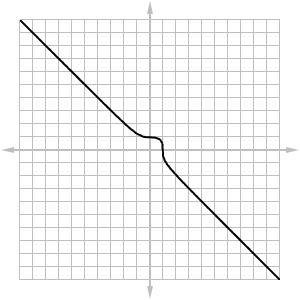
\includegraphics[width=0.6\linewidth]{implicit7}
            \end{center}
      \item $ \sin^2 y + \cos^2 x = 1 $
            \begin{center}
              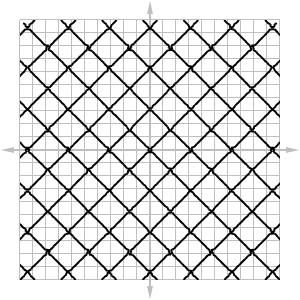
\includegraphics[width=0.6\linewidth]{implicit2}
            \end{center}
      \vfill\null
      \columnbreak
      \item $ x^3 + y^3 = 6xy $ (the folium of Descartes)
            \begin{center}
              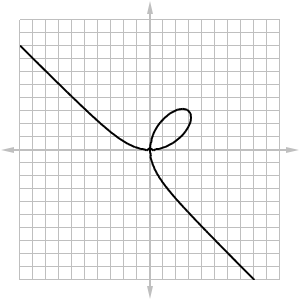
\includegraphics[width=0.6\linewidth]{folium}
            \end{center}
      \item $ y \cos x = 1 + \sin(xy) $
            \begin{center}
              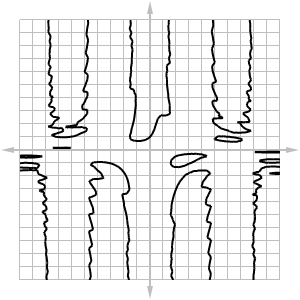
\includegraphics[width=0.6\linewidth]{implicit6}
            \end{center}
      \vfill\null
      \columnbreak
      \item $ x^2 + xy - y^2 = 4 $
            \begin{center}
              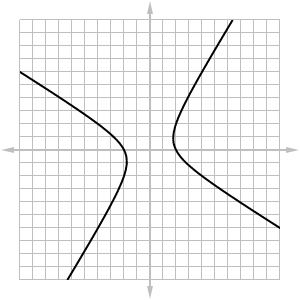
\includegraphics[width=0.6\linewidth]{implicit4}
            \end{center}
      \item $ \frac{1}{x} + \frac{1}{y} = 1 $
            \begin{center}
              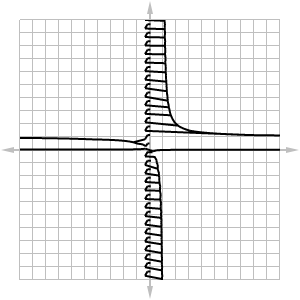
\includegraphics[width=0.6\linewidth]{implicit3}
            \end{center}
      \item $ x^2 y^2 + x \sin y = 4 $
            \begin{center}
              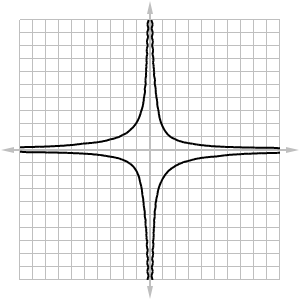
\includegraphics[width=0.6\linewidth]{implicit8}
            \end{center}
      \item $ x^4 y^2 - x^3 y + 2 x y^3 = 0 $
            \begin{center}
              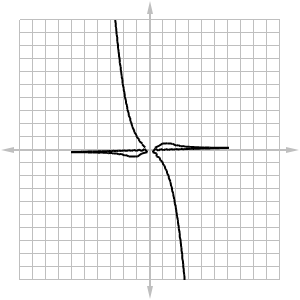
\includegraphics[width=0.6\linewidth]{implicit9}
            \end{center}
      \item $ \tan(x - y) = \frac{y}{1 + x^2} $
            \begin{center}
              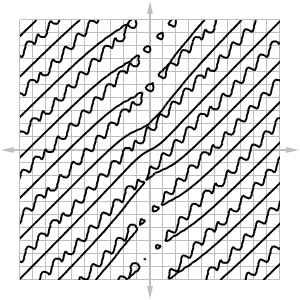
\includegraphics[width=0.6\linewidth]{implicit5}
            \end{center}
      \item $ \sin\left(\frac{x}{y}\right) = \frac{1}{2} $
            \begin{center}
              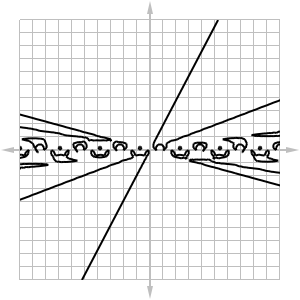
\includegraphics[width=0.6\linewidth]{implicit16}
            \end{center}
    \end{enumerate}
    \end{multicols}
  \item Consider the circle $ x^2 + y^2 = 1 $. Find the equation of the tangent to the curve at $ (\sqrt{2}, \sqrt{2}) $.
  \item The ellipse $ x^2 + 3y^2 = 36 $ has two tangent lines passing through the point $ (12, 3) $. Find both.
        \textit{This question is similar to one from the 2015 Scholarship paper.}
  \begin{multicols}{2}
  \item Find $ x' $ and $ y' $ if $ \ln(y) = \sin(xy) + \frac{x}{y} $.
        \begin{center}
          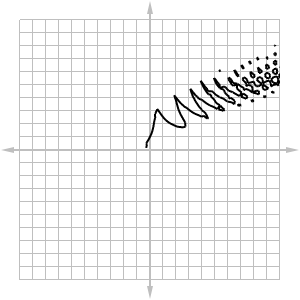
\includegraphics[width=0.6\linewidth]{implicit13}
        \end{center}
  \end{multicols}
  \begin{multicols}{2}
  \item Find $ y'' $ if $ x^4 + y^4 = 16$.
        \begin{center}
          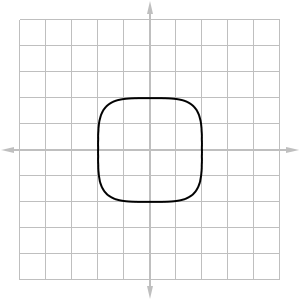
\includegraphics[width=0.6\linewidth]{implicit15}
        \end{center}
  \end{multicols}
  \begin{multicols}{2}
  \item If $ x^2 + xy + y^3 = 1 $, find the value of $ y''' $ at the point where $ x = 1 $.
        \begin{center}
          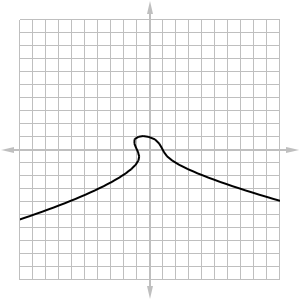
\includegraphics[width=0.6\linewidth]{implicit14}
        \end{center}
  \end{multicols}
  \begin{multicols}{2}
  \item Find a tangent line to the curve $ 2(x^2 + y^2)^2 = 25(x^2 - y^2) $ at the point $ (3, 1) $. This curve is known
        as a lemniscate.
        \begin{center}
          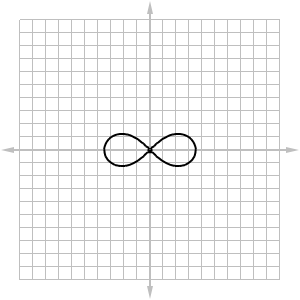
\includegraphics[width=0.6\linewidth]{lemniscate}
        \end{center}
  \end{multicols}
  \begin{multicols}{2}
  \item Find a tangent line to the curve $ y^2(y^2 - 4) = x^2(x^2 - 5) $ at the point $ (0, -2) $. This curve is known
        as a devil's curve.
        \begin{center}
          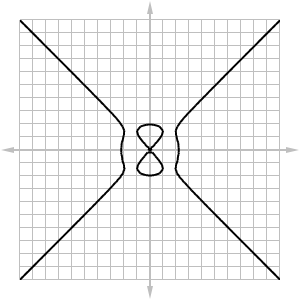
\includegraphics[width=0.6\linewidth]{devilcurve}
        \end{center}
  \end{multicols}
  \item Consider the ellipse $ x^2 - xy + y^2 = 3 $.
    \begin{enumerate}
      \item Find the points where the ellipse crosses the $ x$-axis.
      \item Show that the tangent lines of the curve at these points are parallel.
      \item Find the maximum and minimum points of the curve.
    \end{enumerate}
  \item Consider a circle $ C $ that is tangent to $ 3x + 4y - 12 = 0 $ at $ (0, 3) $ and contains $ (2, -1) $. Set
        up equations that would determine the centre $ (h,k) $ and radius $ r $ of $ C $.
  \item The Bessel function of order 0, $ y = J(x) $, satisfies the equation
        \begin{displaymath}
          xy'' + y' + xy = 2
        \end{displaymath}
        for all values of $ x $. The value of the function at 0 is $ J(0) = 1 $.
    \begin{enumerate}
      \item Find $ J'(0) $.
      \item Use implicit differentiation to find $ J''(0) $.
    \end{enumerate}
  \item Scholarship 2018: Suppose a circle with centre $ O $ is drawn, and a point $ A $ is picked within the circle. Where should a point $ P $ be
        placed on the circumference of the circle such that the interior angle of the triangle $ OAP $ at $ P $ is maximised?
  \item Scholarship 2012: Consider the equation $ x^n = \tan(ny) $, where $ n $ is a constant. Find an expression
        for $ \od{y}{x} $ in terms of $ x $.
  \item Scholarship 2017: The functions $ \sinh $ and $ \cosh $ are defined as follows.
        \begin{align*}
          \sinh x &= \frac{1}{2}\left(e^x - e^{-x}\right),\\
          \cosh x &= \frac{1}{2}\left(e^x + e^{-x}\right).
        \end{align*}
        The inverse function of $ \sinh $ is denoted by $ \sinh^{-1} $. By implicit differentiation, or
        otherwise, show that
        \begin{displaymath}
          \od{}{x} \sinh^{-1} x = \frac{1}{\sqrt{x^2 + 1}}.
        \end{displaymath}
  \item Consider the following family of curves, known as Durer's shell curves (shown here for $ a = 2 $, $ b = 3 $):
        \begin{displaymath}
          (x^2 + xy + ax - b^2)^2 = (b^2 - x^2)(x - y + a)^2.
        \end{displaymath}
        \begin{center}
          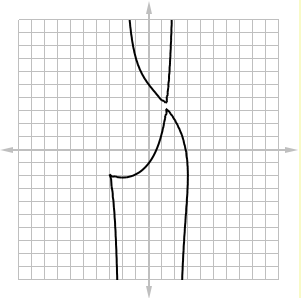
\includegraphics[width=0.3\linewidth]{durer}
        \end{center}
    \begin{enumerate}
      \item For which value(s) of $ b $ does the curve become a straight line?
      \item Suppose that we restrict $ a = \frac{b}{2} $. Find all non-differentiable points on the curve.
    \end{enumerate}
\end{enumerate}

\subsection{References}
For many more examples and exercises, see Stewart, \S2.6. Wikipedia also has a long list of interesting curves
at \url{https://en.wikipedia.org/wiki/List_of_curves}.

For a proof of the implicit function theorem, see Loomis and Sternberg, \S3.11.

This subject properly belongs to the field of differential geometry; see the references for \S9.

\subsection{Homework problems}
\begin{enumerate}
  \item Find $ y' $ in each case:
    \begin{multicols}{3}
    \begin{enumerate}
      \item $ y^2 = x^3 + 3x^2 $\\(Tschirnhausen cubic)
            \begin{center}
              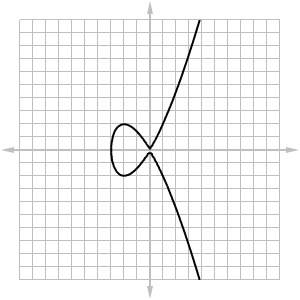
\includegraphics[width=\linewidth]{implicit10}
            \end{center}
      \item $ \sin(x + y) = 2x - 2y $
            \begin{center}
              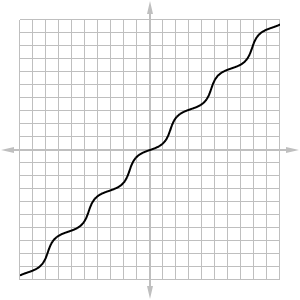
\includegraphics[width=\linewidth]{implicit11}
            \end{center}
      \item $ y^2 = 5x^4 - x^2 $\\(kampyle of Eudoxus)
            \begin{center}
              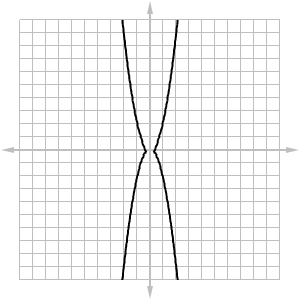
\includegraphics[width=\linewidth]{implicit12}
            \end{center}
    \end{enumerate}
    \end{multicols}
  \item Find the equation of the normal line to the curve $ x^2 + 2xy - y^2 + x = 2 $ at the point $ (1, 2) $.
  \item Show that the sum of the $ x $ and $ y $ intercepts of any tangent line to the curve $ \sqrt{x} + \sqrt{y} = \sqrt{c} $
        is just $ c $.
\end{enumerate}
